\documentclass{article}
\usepackage{amsmath,amssymb}
\usepackage[numbers]{natbib}
\usepackage{geometry}
 \geometry{
 a4paper,
 total={170mm,257mm},
 left=30mm,
 top=30mm,
 right=30mm,
 bottom=30mm
 }
 
\usepackage{graphicx}
\usepackage{caption}
\usepackage{subcaption}
\usepackage{float}

\usepackage{hyperref}
\hypersetup{%
  colorlinks=true,% hyperlinks will be coloured
}

\setlength{\parskip}{1em}

\title{Reinforcement Learning Assignment-5 \\
	\Large Function Approximation, Policy Gradients and Deep Reinforcement Learning \\}
\begin{document}
\author{Utkarsh Prakash \\ \normalsize 180030042}
\maketitle
\section{OpenAI Gym Environments Considered}
    \subsection{Mountain Car}
    A car is on a one-dimensional track, positioned between two "mountains". The goal is to drive up the mountain on the right; 
    however, the car's engine is not strong enough to scale the mountain in a single pass. Therefore, the only way to succeed is to 
    drive back and forth to build up momentum. \par

    \noindent %The next paragraph is not indented
    The state of the car is decided by the position of the car along the horizontal axis and the velocity. At the beginning of the
    episode, the car starts from the bottom of the hills (valley). The episode ends when the car reaches the goal or after
    200 steps (which ever is earlier). The action space consists of 3 actions: \{push left, push right, do nothing\}. A negative reward
    of $-1$ is applied at each timestep. The objective of the car is to reach the top of the hill on the right as early as possible, 
    because at each timestep it will be rewarded negatively. \par

    \begin{figure}[H]
        \graphicspath{ {../tmp/} }
        \begin{center}
        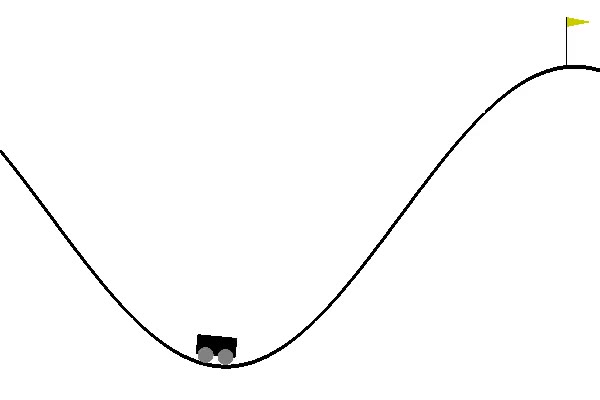
\includegraphics[width=8cm]{mountain_car.jpg}
        \end{center}
        \caption{MountainCar. For more details click \href{https://gym.openai.com/envs/MountainCar-v0/}{here} }
        \label{mountain_car}
    \end{figure}

    \subsection{CartPole}
    A pole is attached by an un-actuated joint to a cart, which moves along a frictionless track. The system is controlled by applying a 
    force of +1 or -1 to the cart. The pendulum starts upright, and the goal is to prevent it from falling over. A reward of +1 is provided for
    every timestep that the pole remains upright. The episode ends when the pole is more than 15 degrees from vertical, or the cart moves more 
    than 2.4 units from the center or the length of the episode is atleast 200.\par
    
    \begin{figure}[H]
        \graphicspath{ {../tmp/} }
        \begin{center}
        
\includegraphics[width=8cm]{cartpole.png}
        \end{center}
        \caption{CartPole. For more details click \href{https://gym.openai.com/envs/CartPole-v1/}{here} }
        \label{policy_iter_jack_problem}
    \end{figure}
    
    \noindent %The next paragraph is not indented
    The state of the cart is decided by it's position (x), velocity (x\_dot), pole angle (theta) and pole angular velocity (theta\_dot). The action space
    consists of 2 actions: \{push left, push right\}.

\section{Linear Function Approximation}
    \subsection{Mountain Car}
        \subsubsection{Tile Coding}
        We consider a grid of 14 x 14 tiling i.e. each tiling consists of 196 tiles and we have $n=7$ such tilings. The offsets for these tilings were:
        [(0, 0), (0.018, 0.004), (0.036, 0.008), (0.055, 0.013), (0.073, 0.017), (0.092, 0.021), (0.110, 0.025)], where the first and second dimension represents 
        the position and velocity of the car respectively. We run Q-Learning and SARSA algorithm for $5,000$ episodes and 
        average the results over $2$ runs. The $\epsilon$ or the exploration factor in the $\epsilon$-greedy policy is chosen to be $0.8$ initially and is 
        decreased by a factor of $0.99$ after every epsiode. This ensures that each of the state is explored infinitely often. The learning rate or the step-size 
        $(\alpha)$ and discount factor $(\gamma)$ are chosen to $0.3/n$, where $n$ is the number of tiling and $0.99$ respectively. We use a constant step-size.
        The comparison between the average episodic rewards for both the algorithms is shown in Fig. \ref{mountaincar_tile}.

        \subsubsection{Radial Basis Function Coding}
        We represent the state space using 22 x 22 equally spaced RBF centers with a width of $0.000486$ which is the square of half of the distance between two 
        adjacent centers. We run Q-Learning and SARSA algorithms for $2,000$ episodes and average the results over $2$ runs. The learning rate or the step-size 
        $(\alpha)$ is set to $0.05$. Rest of the setting is similar to tile coding. The comparison between the average episodic rewards for both the algorithms 
        is shown in Fig. \ref{mountaincar_radial}.

        \begin{figure}[H]
            \graphicspath{ {../Experiments/Linear_Function_Approximation/} }
            \centering
            \begin{subfigure}{.5\textwidth}
              \centering
              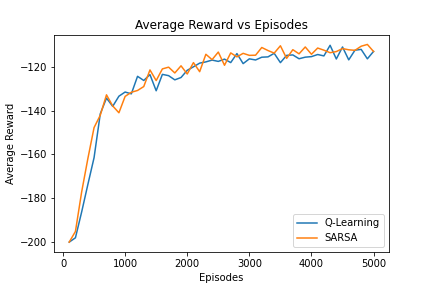
\includegraphics[width=\linewidth]{Mountaincar_tile.png}
              \caption{Tile Coding}
              \label{mountaincar_tile}
            \end{subfigure}%
            \begin{subfigure}{.5\textwidth}
              \centering
              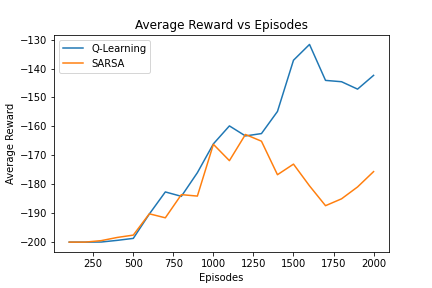
\includegraphics[width=\linewidth]{Mountaincar_radial.png}
              \caption{Radial Basis Function Coding}
              \label{mountaincar_radial}
            \end{subfigure}
            \caption{Average episodic reward as a function of episodes for Mountain Car.}
            \end{figure}
        
        \noindent %The next paragraph is not indented
        \textbf{Conclusion:} \\
          Tile coding seems to be performing better than the Radial Basis Function coding 
          as the former achieves a higher average episodic rewards. Moreover, the learning is 
          also much stable while using Tile Coding than the RBF coding. The computational cost 
          of RBF coding is significantly higher than that of Tile coding as the former 
          requires computation of the costly RBF function as opposed to one-hot calculation in
          the latter.  

    \subsection{CartPole}
        For this section, we consider the position (x) $\in [-3, 3]$, velocity (x\_dot) $\in [-3.5, 3.5]$, pole angle (theta) $\in [-0.25, 0.25]$ and 
        pole angular velocity (theta\_dot) $\in [-3.5, 3.5]$.

        \subsubsection{Tile Coding}
        We consider a hyper-grid of 22 x 22 x 22 x 22 tiling i.e. each tiling consists of $22^{4}$ tiles and we have $n=4$ such tilings. The offsets for these 
        tilings were: [(0, 0, 0, 0), (0.07, 0.23, 0.03, 0.55), (0.14, 0.48, 0.06, 1.11), (0.20, 0.71, 0.08, 1.67)], where the dimensions represent position (x), 
        velocity (x\_dot), pole angle (theta) and pole angular velocity (theta\_dot) of the cart respectively. We run Q-Learning and SARSA algorithm for $1,000$ episodes and 
        average the results over $2$ runs. The $\epsilon$ or the exploration factor in the $\epsilon$-greedy policy is chosen to be $0.8$ initially and is 
        decreased by a factor of $0.99$ after every epsiode. This ensures that each of the state is explored infinitely often. The learning rate or the step-size 
        $(\alpha)$ and discount factor $(\gamma)$ are chosen to $0.1/n$, where $n$ is the number of tiling and $0.99$ respectively. We use a constant step-size.
        The comparison between the average episodic rewards for both the algorithms is shown in Fig. \ref{cartpole_tile}.

        \subsubsection{Radial Basis Function Coding}
        We represent the state space using 15 x 15 x 15 x 15 equally spaced RBF centers with a width of $0.02918403$ which is the square of half of the distance between two 
        adjacent centers. We run Q-Learning and SARSA algorithms for $1,000$ episodes and average the results over $1$ runs. The learning rate or the step-size 
        $(\alpha)$ is set to $0.1$. Rest of the setting is similar to tile coding. The comparison between the average episodic rewards for both the algorithms is shown in 
        Fig. \ref{cartpole_radial}.

        \begin{figure}[H]
            \graphicspath{ {../Experiments/Linear_Function_Approximation/} }
            \centering
            \begin{subfigure}{.5\textwidth}
              \centering
              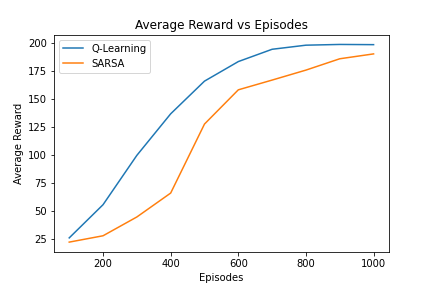
\includegraphics[width=\linewidth]{Cartpole_tile.png}
              \caption{Tile Coding}
              \label{cartpole_tile}
            \end{subfigure}%
            \begin{subfigure}{.5\textwidth}
              \centering
              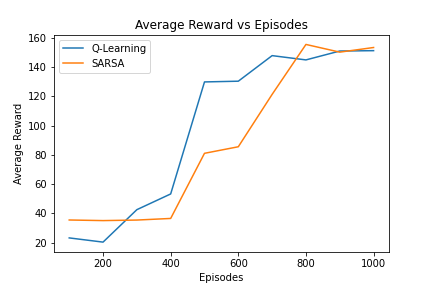
\includegraphics[width=\linewidth]{Cartpole_radial.png}
              \caption{Radial Basis Function Coding}
              \label{cartpole_radial}
            \end{subfigure}
            \caption{Average episodic reward as a function of episodes for CartPole.}
            \end{figure}

        \noindent %The next paragraph is not indented
        \textbf{Conclusion:} \\
        Tile coding seems to be performing better than the Radial Basis Function coding. Although we ran the RBF coding 
        only for 1 run due to its high computational cost, we expect the results to be similar for multiple runs. The 
        computational cost of RBF coding for CartPole was significantly higher than in Mountain Car because we had 4-dimensional state space.
        Moreover, we can see that with Tile coding, both Q-Learning and SARSA could reach near perfect score of $200$.  

\section{REINFORCE Algorithm}
    In this section we compare the performance
    of different versions of the REINFORCE algorithms which differ in their policy gradient calculations, as described below:
    \begin{equation}
        \nabla \rho(\theta) = \mathbb{E}_{\tau} \left [\left ( \sum_{t=0}^{T} \nabla_{\theta} log \pi (a_{t} | s_{t}) \right) \left ( \sum_{t=0}^{T} \gamma^{t} R_{t} \right) \right ]
    \label{reinforce}
    \end{equation}

    \begin{equation}
        \nabla \rho(\theta) = \mathbb{E}_{\tau} \left [\left ( \sum_{t=0}^{T} \nabla_{\theta} log \pi (a_{t} | s_{t}) \left ( \sum_{k=t+1}^{T} \gamma^{k-t-1} R_{k} \right) \right) \right ]
    \label{reinforce_variance}
    \end{equation}
    Let's call the version of the algorithm described by \ref{reinforce} and \ref{reinforce_variance} as \textbf{REINFORCE} and \textbf{REINFORCE\_var} respectively.
    We benchmark the performance of both the algorithms on standard Mountain Car and CartPole tasks. 

    \subsection{Mountain Car}
    We parameterize the policy using a neural network consisting of 4, 16 and 2 units in the input, hidden and output layer. We use ReLU and softmax activation for
    the first and second layer respectively. We run each of the algorithm for $5,000$ episodes. 
    The learning rate or the step-size $(\alpha)$ used is fixed and equals $0.01$. The discount factor $(\gamma)$ is chosen to be $0.99$. \par

    \noindent %The next paragraph is not indented
    We observe that for both of the algorithms the average episodic rewards always stays the same i.e. $-200$. We also tried to increase the number of steps per episode to
    $1000$ but the effect was similar. Another thing we tried was to make the policy network deeper with more units in each layer. More specifically, we used a similar
    network as above but with 2 hidden layers each with $64$ units. However, the network didn't seem to learn anything. We conjecture that this behaviour is observed 
    due to training the network for very little number of episodes. Given enough number of episodes the
    network should be able to learn because Mountain Car is a difficult problem because the agent at each timestep is penalized for not reaching the goal position and the
    learning can be difficult initially.

    \subsection{CartPole}
    We parameterize the policy using a neural network consisting of 4, 16 and 2 units in the input, hidden and output layer. We use ReLU and softmax activation for
    the first and second layer respectively. We run each of the algorithm for $5,000$ episodes and average the results over $2$ runs. 
    The learning rate or the step-size $(\alpha)$ used is fixed and equals $0.01$. The discount factor $(\gamma)$ is chosen to be $0.99$. The comparison of average 
    episodic rewards for both of the algorithms is shown in Fig. \ref{cartpole_reinforce}.
    
    \begin{figure}[H]
        \graphicspath{ {../Experiments/Linear_Function_Approximation/} }
        \begin{center}
        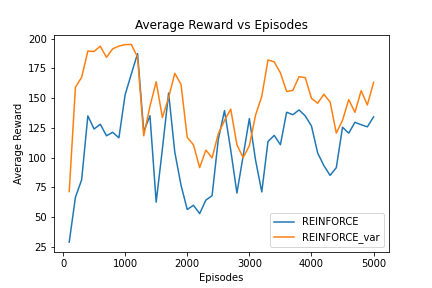
\includegraphics[width=8cm]{Cartpole_reinforce.png}
        \end{center}
        \caption{Average episodic reward as a function of episodes for CartPole problem using different versions of REINFORCE algorithm.}
        \label{cartpole_reinforce}
    \end{figure}

    \noindent %The next paragraph is not indented
    \textbf{Conclusion:} \\
    The REINFORCE\_var version seems to be performing better than the vanilla version of the REINFORCE algorithm. This can be
    attributed to the fact that the variance of the policy gradient estimate is lower in the REINFORCE\_var version than the
    vanilla one, which makes the learning more stable. If we would averaged over a lot of multiple runs, the effect of lower
    variance would have been more pronounced. Moreover, we also observe that REINFORCE\_var achieves near perfect score of $200$.
    
\section{Deep Reinforcement Learning}
    In this section we compare the performance of Advantage Actor Critic method (A2C) and Deep Q-Network (DQN) on the standard CartPole task. The comparison of average episodic 
    rewards for both of the algorithms is shown in Fig. \ref{cartpole_deeprl}.
    \subsection{Advantage Actor Critic (A2C)}
    The Actor network comprises of 1 input, 2 hidden and 1 output layers. The input, first hidden, second hidden and output layer comprises of 4, 64, 64 and 2 units respectively.
    We use ReLU activation function apart from the last layer where we use softmax activation.
    The Critic network is same as the Actor network apart from the output layer which consists of 1 output unit and no activation. We train both the networks for $4,000$ episodes using Adam 
    optimizer with a learning rate of $0.001$ and set rest of the hyperparameters to their default values. The discount factor $(\gamma)$ was set to $0.99$.

    \subsection{Deep Q-Network (DQN)}
    The DQN network consists of 1 input, 2 hidden and 1 output layers. The input, first hidden, second hidden and output layer comprises of 4, 64, 64 and 2 units respectively.
    We use ReLU activation function apart from the last layer where no activation function is used. We train the network for $4,000$ episodes using Adam optimizer with a learning rate of $0.0005$ 
    and rest of hyperparameters were set to their default values. We update the network after every $4$ timesteps by choosing a batch of $64$ experiences from a buffer of size $10^{5}$.
    The $\epsilon$ or the exploration factor 
    in the $\epsilon$-greedy policy is chosen to be $1.0$ initially and is decreased by a factor of $0.995$ after every epsiode but we ensure that it never falls below $0.01$. This ensures
    that each of the state is explored infinitely often. The discount factor $(\gamma)$ was set to $0.99$.
    
    \begin{figure}[H]
        \graphicspath{ {../Experiments/Linear_Function_Approximation/} }
        \begin{center}
        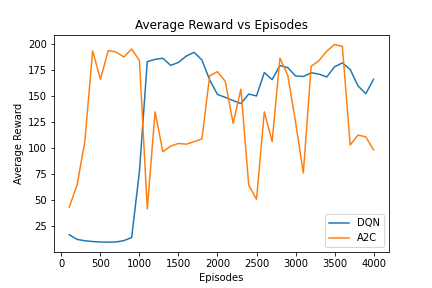
\includegraphics[width=8cm]{Cartpole_deeprl.png}
        \end{center}
        \caption{Average episodic reward as a function of episodes for CartPole problem using different Deep Reinforcement Learning algorithms.}
        \label{cartpole_deeprl}
    \end{figure}

    \noindent %The next paragraph is not indented
    \textbf{Conclusion:} \\
    The learning seems to be more stable with DQN as compared to A2C. This can be due to the fact that in A2C we have two networks with different
    roles and we utilize the estimates of the critic to update the actor, which may have a wrong estimates. However, we can observe that both the algorithms are 
    able to achieve a near perfect score of $200$.
    
\section{Conclusion}
\begin{itemize}
\item The added computational cost of RBF coding doesn't provide any real benefit and Tile coding seems to work better than Radial Basis Function coding.
\item Q-Learning performs at par or better than SARSA. This is due to the fact the Q-Learning is an off-policy learning algorithm where our target policy
is the optimal policy whereas SARSA is an on-policy algorithm.
\item REINFORCE\_var performs better than REINFORCE algorithm because of lesser variance of the policy gradient estimator of the former.
\item DQN and A2C methods perform equally well, however the learning is more stable with the former.
\item In general, if we compare the performance in previous assignment to this assignment, we observe function approximation tends to give better results. 
\end{itemize}

\end{document}